\chapter{Introduction} \label{chapter:introduction}

\section{Motivation }

\begin{figure}[h]
    \begin{center}
        \begin{tabular}{@{\hspace{0.1cm}}c}
           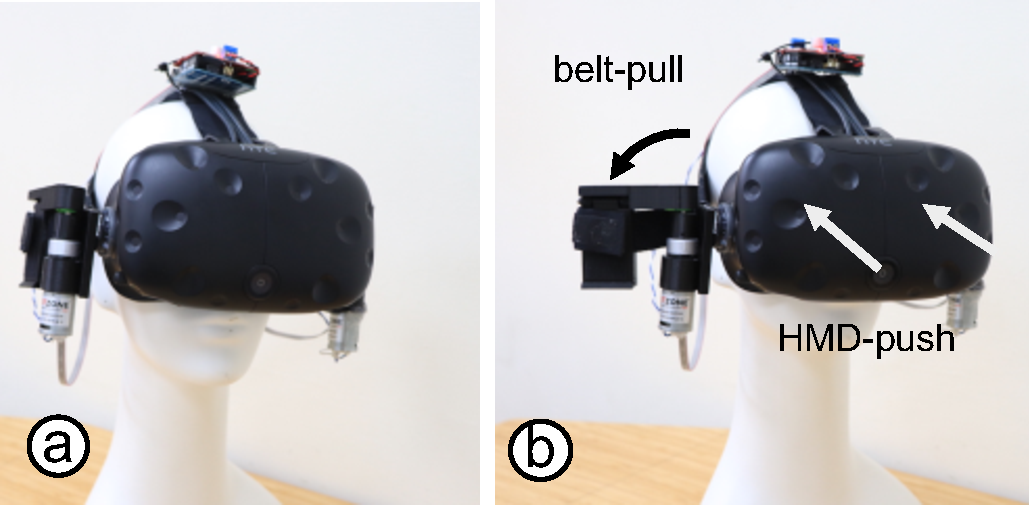
\includegraphics[width=1\textwidth]{figures/FacePush.pdf}
        \end{tabular}
        \captionof{figure}{(a) FacePush presents a pulley system incorporated with HMD providing pressure on face. (b) Our system pulls the belts of the HMD to generate discrete/continuous and weak/strong pressure stimuli to enhance}
        \label{fig:FacePush Intro}
    \end{center}
\end{figure}

Simulated haptics is a key component to enhance immersion in virtual environments. Prior research has proposed various mechanisms to generate different modes of haptic feedback. While many were deployed on limbs, e.g., through wearable interfaces \cite{Impacto} or handheld controllers \cite{normalTouch, hapticLink}, recent research has started to explore simulating haptics directly through Head-Mounted Displays (HMDs),  such as the introduction of thermal \cite{ThermoVR, Ambiotherm}, vibrotactile \cite{HapticHead} and force \cite{GyroVR, HangerOVER} feedback on users' head or face.

\section{FacePush }

In line with such efforts, we present \textit{FacePush}, an HMD integrated with a pulley system that can manipulate the HMD in order to enable pressure to be applied upon the user's head resulting in a normal force on the user's face. The mechanism of FacePush is achieved by a shifting torque provided by the two motors to a facial normal force (Figure \ref{fig:FacePush Intro}(a-b)). By controlling the angles of the motors, FacePush can generate normal forces with varying strengths. 

\begin{figure}[hp]
    \begin{center}
        \begin{tabular}{@{\hspace{0.1cm}}c}
           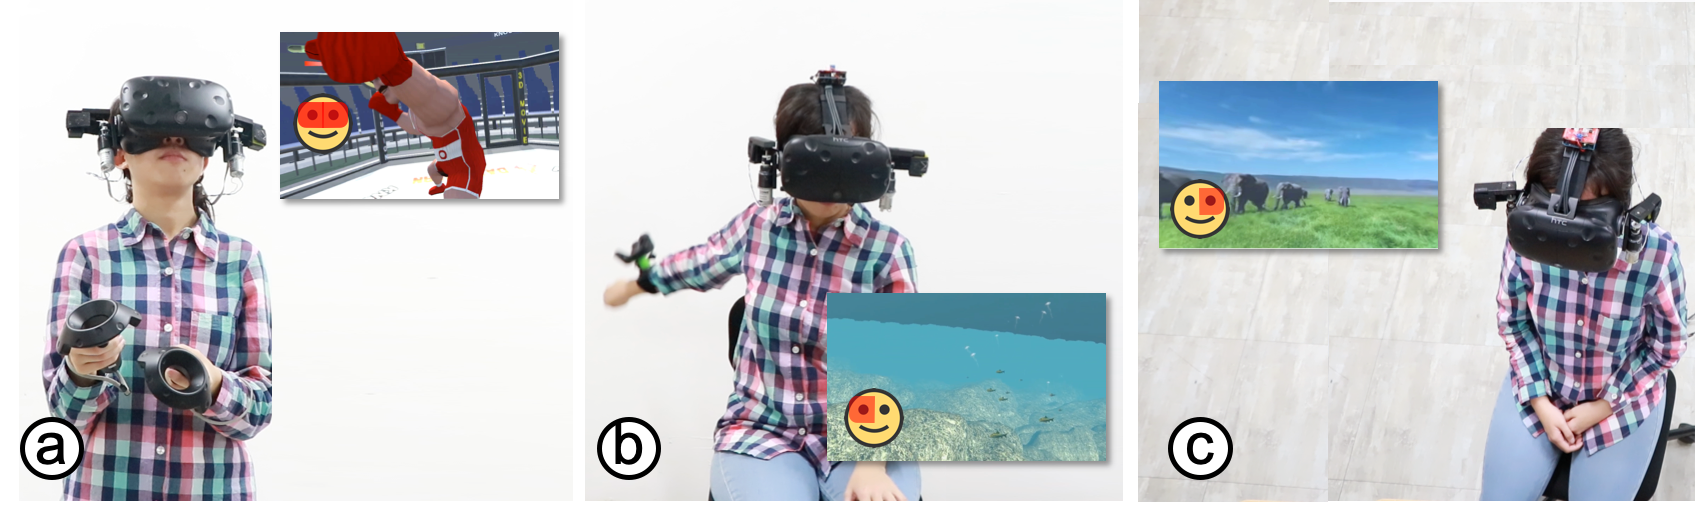
\includegraphics[width=1\textwidth]{figures/3Applications.png}
        \end{tabular}
        \captionof{figure}{(a) Boxing (b) Diving and (c) Attention guidance experiences in virtual environments. In (a)(b)(c), the face icons indicate the displayed force on face.}
        \label{fig:3Applicaions Intro}
    \end{center}
\end{figure}

FacePush allows an improvement in the sense of presence for example applications such as boxing (Figure \ref{fig:3Applicaions Intro}(a)) and underwater swimming (Figure \ref{fig:3Applicaions Intro}(b)). We also use normal force as a directional cue for direction guidance in 360 degree videos (Figure  \ref{fig:3Applicaions Intro}(c)).



\section{Contribution }

As such, FacePush offer three main contributions, namely: (1) an HMD integrated with a pulley system to render the haptic sensations via normal force acting on a user's face; (2) studies determining ADT and JND which inform effective design of noticeable and discernible normal force, along with ratings of user comfort; and (3) three applications which demonstrate use of discrete and continuous normal force that enhance user experience and offer a means to convey direction guidance.